  \documentclass[10pt,twocolumn,letterpaper]{article}

\usepackage{cvpr}
\usepackage{times}
\usepackage{epsfig}
\usepackage{graphicx}
\usepackage{amsmath}
\usepackage{amssymb}
\usepackage{algorithm}
\usepackage{algpseudocode}

% Include other packages here, before hyperref.

% If you comment hyperref and then uncomment it, you should delete
% egpaper.aux before re-running latex.  (Or just hit 'q' on the first latex
% run, let it finish, and you should be clear).
\usepackage[pagebackref=true,breaklinks=true,letterpaper=true,colorlinks,bookmarks=false,draft]{hyperref}

% \cvprfinalcopy % *** Uncomment this line for the final submission

\def\cvprPaperID{****} % *** Enter the CVPR Paper ID here
\def\httilde{\mbox{\tt\raisebox{-.5ex}{\symbol{126}}}}

% Pages are numbered in submission mode, and unnumbered in camera-ready
\ifcvprfinal\pagestyle{empty}\fi
\begin{document}

%%%%%%%%% TITLE
\title{Deformable Diversity Similarity for Partial Matching of 3D Shapes}

\author{First Author\\
Institution1\\
Institution1 address\\
{\tt\small firstauthor@i1.org}
% For a paper whose authors are all at the same institution,
% omit the following lines up until the closing ``}''.
% Additional authors and addresses can be added with ``\and'',
% just like the second author.
% To save space, use either the email address or home page, not both
\and
Second Author\\
Institution2\\
First line of institution2 address\\
{\tt\small secondauthor@i2.org}
}

\maketitle
%\thispagestyle{empty}

%%%%%%%%% ABSTRACT
\begin{abstract}
We propose a novel approach for the matching of partial deformable shapes in 3D. Inspired by recent advances in 2D template matching techniques, our method relies on the concept of deformable diversity similarity(DDIS), extends and adapts it from an image to the 3D shape domain, and leverages the distinct behavior of this framework in different scales to achieve shape correspondences. We evaluate this framework on the SHREC16 partial matching of deformable shapes and show state of the art performance in achieving sparse correspondences.
\end{abstract}

%%%%%%%%% BODY TEXT
\section{Introduction}

%%%%%%%%%%%%%%%%%%%%%%%%%%%%%%%%%%%%%%%%%%%%%%%%%%%%%%%%%%%%%%%%%%%%%%%Problem Definition
Shape correspondence is a fundamental and challenging problem in computer vision and graphics. It has usage in various applications such as transferring texture and animation. 
Shapes rarely, if ever manifest in only one pose. While rigid transformations between surfaces is a well researched topic with many adequate solutions, a more challenging problem arises when a shape is deformed non-rigidly, a case all too common for people, animals and objects.
Moreover, the shape acquisition process almost always lead to partiality of the scanned object. Occlusions arise from different angles of acquisition, which cause an object to occlude itself, or stem from other occluding objects. 
An additional type of difficulty which might be occur is topological noise, occurring when shapes touch pn another, thus making  sensors unable to seperate them.
All of these combined give rise to the challenging problem of partial correspondences, where a deformed and incomplete shape, possibly with topological changes, has to be matched with its full version. The goal of this paper is to deal with this challenging problem.

%%%%%%%%%%%%%%%%%%%%%%%%%%%%%%%%%%%%%%%%%%%%%%%%%%%%%%%%%%%%%%%%%%%%%%%Previous Works
While in a rigid setting the problem can be solved by RANSAC and ICP like approaches\cite{rusu2009fast, holz2015registration}, extending these to non-rigid case produces mediocre results due to an underlying assumption of small deformations. 
%%%%Isometry based methods
Early methods specialized for the non-rigid problem focused on minimization of intrinsic metric distortion\cite{bronstein2006generalized,Torsello:2012:GAD:2354409.2354702} and regularity of parts\cite{Bronstein:2009:PSO:1553357.1553368,bronstein2008not}. These methods all contain with them a global assumption of isometry which holds only approximately, these tended to break down with it, and are also unable to handle extreme partiality. 
%%functional correspondences
Another family of method is based on functional correspondence. These methods model correspondences as a linear operator of a known nature between a space of functions on manifolds\cite{Ovsjanikov:2012:FMF:2185520.2185526}. These methods, originally designed for the full shape correspondence scenario have achieved state of the art results on various partial matching tasks in the recent years\cite{litany2017fully,vestner2017efficient,rodola2017partial}, and produce dense correspondence maps, but are not parallelizable, and their reliance on intrinsic metrics makes them invariant to symmetry. 

%%%%%%%%%%%%%%%%%%%%%%%%%%%%%%%%%%%%%%%%%%%%%%%%%%%%%%%%%%%%%%%%%%%%%%%Our key ideas
We take a different approach. We take advantage of the fact that while the isometric property tends to break over large distances, it usually holds approximately in limited environments. These also tend to suffer a lot less from boundary effects, especially when concentrated around the extremities of a shape. 

We can thus treat the problem of partial correspondences as matching of multiple templates, each smaller then the partial surface centered around shape landmarks. 

In addition, since point descriptors are known to be modified by partiality and deformations, instead of using them directly, we follow the approach of\cite{talmi2017template}(\textbf{DDIS}) which tackles template matching in 2D and use simple statistical assumptions on the nature of nearest neighbors between small patch descriptors, along with the assumption of an approximate conservation of distances in medium environments to obtain similarity scores between these partial shape templates.

We analyze the behavior of DDIS similarity in different scales and devise a multi scale scheme which leverages the advantages of each scale while masking their shortcomings.

%%%%%%%%%%%%%%%%%%%%%%%%%%%%%%%%%%%%%%%%%%%%%%%%%%%%%%%%%%%%%%%%%%%%%%%Our improvements
We show that using this approach, we are able to generate a set of sparse correspondences, which are less prone to symmetrical assignment than functional correspondence reliant methods, and are of superior quality on the SHREC16 Partial matching challenge\cite{cosmo2016shrec}. We then demonstrate how these sparse correspondences can be used as an input to existing functional correspondence algorithms to obtain dense correspondences or a higher quality.
%%%%%%%%%%%%%%%%%%%%%%%%%%%%%%%%%%%%%%%%%%%%%%%%%%%%%%%%%%%%%%%%%%%%%%%Our Contributions
In summary, our contributions are:
\begin{itemize}
	\item A non trivial extension of Deformable Diversity from 2 to 3 Dimensions.
	\item A modified DDIS similarity measure which is more well suited to handle matching of templates with a different number of points.
	\item An empirical analysis of DDIS behavior in different scales, leading to an improved multi-scale framework.
	\item A novel multi-template approach to partial matching of deformable shapes which can both produce state of the art sparse correspondences, and be used as an input to functional correspondence algorithms, significantly improving the results obtained by these.
\end{itemize}

The rest of the work is organized as follows: in section 2 we go over related works in the field of shape analysis. Section 3 introduces our Deformable Diversity framework for 3D shape matching. Experiments and results are given in section 4, and the conclusions are in section 5.

%%%%%%%%%%%%%%%%%%%%%%%%%%%%%%%%%%%%%%%%%%%%%%%%%%%%%%%%%%%%%%%%%%%%%%%
%%%%%%%%%%%%%%%%%%%%%%%%%%%%%%%% section: Related work
%%%%%%%%%%%%%%%%%%%%%%%%%%%%%%%%%%%%%%%%%%%%%%%%%%%%%%%%%%%%%%%%%%%%%%%

\section{Related work}\label{chap:related work}


\subsection{Matching Of Deformable Surfaces}
%%[APL15] [MDK16] [SPKS16][VLR17][OBCS12][KBB13][PBB13b][KBBV15][HWG14]
%%%%%%%%%%%%%%%%%%%%%%%%%%%%%%%%%%%%%%%%%Shape Descriptors%%%%%%%%%%%%%%%%%%%%%%%%%%%%%%%%%%%%%%%%%%%%%%%%
As a fundamental problem in computer graphics and vision, an extensive body of work have been done on the matching of surfaces.
A variety of shape descriptors have been devised for this task which can be roughly divided in to 2 families. 
Extrinsic ones, such as PFH\cite{rusu2008learning}, SHOT\cite{tombari2010unique} and FPFH\cite{rusu2009fast} which are usually calculated in euclidean space and are thus sensitive to non rigid deformations, but can discern between reflections and are also more robust to noise, topological artifacts and boundary effects.
On the other hand intrinsic features such as Heat\cite{bronstein2010scale} and Wave Kernel signatures\cite{aubry2011wave} are invariant under isometric transformations, but are very sensitive to partiality and are unable to discern between symmetric parts.
These have been commonly used to generate rough correspondences between surfaces and point clouds based on their similarity, but are noisy and offer little in terms of bijectivity and continuity of the solution. a measure of global consistency using these can be achieved by solving an energy minimization of the disimilarity matrices steming from an assignment, and the auction algorithm has been commonly employed for this purpose.
%%%%%%%%%%%%%%%%%%%%%%%%%%%%%%%%%%%%%%%%%Distortion minimization%%%%%%%%%%%%%%%%%%%%%%%%%%%%%%%%%%%%%%%%%%%%%%%%
Other methods use pairwise relations between points such as geodesic distances\cite{sahilliouglu2012minimum,sahilliouglu2012scale,sahillioǧlu2011coarse}, and search for a configuration which minimizes the distortions of these. These methods usually carry a high complexity, both due to calculating the pairwise relations, and the combinatorial configuration search, and are thus either obtain sparse matches\cite{sahilliouglu2012minimum,sahilliouglu2012scale,sahillioǧlu2011coarse} to alleviate this complexity, or used strategies such as coarse to fine solutions.
%%%%%%%%%%%%%%%%%%%%%%%%%%%%%%%%%%%%%%%%%Embedding Space%%%%%%%%%%%%%%%%%%%%%%%%%%%%%%%%%%%%%%%%%%%%%%%%
Another common approach has been to embed the shapes into a different lower dimension "canonical"  space, this has been done by generalized MDS\cite{bronstein2006generalized}, an embedding into the mobius group\cite{lipman2009mobius}, or by representation in the LBO basis\cite{shtern2014matching}
 %%%%%%%%%%%%%%%%%%%%%%%%%%%%%%%%%%%%%%%%%Functional Correspondences%%%%%%%%%%%%%%%%%%%%%%%%%%%%%%%%%%%%%%%%%%%%%%%%
 A notable family of works are derived from functional correspondences. Introduced at\cite{Ovsjanikov:2012:FMF:2185520.2185526,pokrass2013sparse,kovnatsky2015functional,vestner2017efficient} these assume that functions can be mapped from one manifold to another via a linear operator, finding this transfer operator allows to embed point in a space where the ICP method can obtain correspondences. 
%%%%%%%%%%%%%%%%%%%%%%%%%%%%%%%%%%%%%%%%%Learning%%%%%%%%%%%%%%%%%%%%%%%%%%%%%%%%%%%%%%%%%%%%%%%%
Lately there has been a large body of works which employ learning methods such as Random Forests\cite{Rodola:2014:DNS:2679600.2679987} and deep learning architectures\cite{masci2016geometric,boscaini2016learning,monti2017geometric}. These show the promise of achieving state of the art performance, but require a lot of annotated data.

\subsection{Partial Matching of Deformable shapes}
The introduction of partiality adds complications which ar not present in the full correspondence scenario. Spectral quantities change drastically, while geodesic paths disappear.
%%%%%%%%%%%%%%%%%%%%%%%%%%%%%%%%%%%%%%%%%Rigid partial matching%%%%%%%%%%%%%%%%%%%%%%%%%%%%%%%%%%%%%%%%%%%%%%%%
For the rigid setup, the Iterative Closest Point(ICP)\cite{Aiger:2008:CSR:1360612.1360684} algorithm, preceded by initial alignment\cite{rusu2008towards} tackle partial matching successfully. Adapting this to the rigid setup however has proved to have limited success due to the alignment which is necessary, and thus is only fit for very small non-rigid deformation.

Early works which were designed with partial matching in mind\cite{bronstein2008not,bronstein2009partial} formulated an energy minimization problem over metric distortion and regularity of corresponding parts. Following works relaxed the regularity requirement by allowing for sparse correspondences\cite{Torsello:2012:GAD:2354409.2354702,rodola2013elastic}. 
Other works\cite{sahilliouglu2012scale,sahilliouglu2012minimum} minimized the distortion metric over the shape extremities by doing combinatorial search of least distortion matches and then densify them while employing a refining scheme in the process. 

In\cite{pokrass2013partial} a bag of words point-wise descriptors on a part in conjunction with a constraint on area similarity and the regularity of the boundary length to produce correspondence less matching parts without point to point correspondences by energy minimization.

Another line of works employ machine learning techniques to learn correspondences between manifolds. 
Recently \cite{rodola2017partial} had proven that partiality induces a slanted diagonal structure in the correspondence matrix and found the Laplacian eigenfunctions from each basis which induces this structure. Current state of the art\cite{litany2017fully} uses this notion in conjunction with joint diagnolization. The main drawback of this method, shared with other intrinsic methods, is its invariance to symmetries. 

\textbf{3D Shape Descriptors} 

%%%%%%%%%%%%%%%%%%%%%%%%%%%%%%%%%%%%%%%%%%%%%%%%%%%%%%%%%%%%%%%%%%%%%%%
%%%%%%%%%%%%%%%%%%%%%%%%%%%%%%%% section: 2D Shape Matching
%%%%%%%%%%%%%%%%%%%%%%%%%%%%%%%%%%%%%%%%%%%%%%%%%%%%%%%%%%%%%%%%%%%%%%%

\subsection{Template matching in 2D}
Template matching in 2D is a well researched topic. Similarly to 3D objects are going complex deformations of pose, and are only seen partially depending on the camera point of view. Recently a series of works which use a very simplistic framework based on the statistical properties of nearest neighbors in low level feature space had made good strides in tackling this complex task.

\textbf{Best Buddies Similarity}
Great strides had been achieved in the field of 2D template matching. Best Buddies Similarity\cite{dekel2015best} is a simple framework which employs a statistical assumption - if two regions $\mathcal{N}$,$\mathcal{M}$ contain the same template patches should maintain Bi Directional Similarity. 
That is - given a point $n_i\in\mathcal{N}$ and a corresponding point $m_i\in\mathcal{M}$ they should point too each other as nearest neighbors - that is if $NN_{\mathcal{M}}(n_i)=m_j$ then on a matching template we should expect $NN_{\mathcal{N}}(m_j)=n_i$. Solving for a matching template then amounts to finding the region which has the highest count of best buddies. This amazingly simple scheme has been show to be able to handle occlusions, missing parts and complex deformations of templates.

\textbf{Deformable Diversity Similarity}
Building upon the above work, \cite{talmi2017template}  relaxed the requirement for a best buddy relation, and added a requirement for spatial coherency.

The rather cumbersome best buddy relation has been relaxed to requiring only that the diversity of the set of nearest neighbors sets between corresponding templates should be high. This is actually prerequisite to a high best buddies similarity score and serves as a rough approximation of it. For this end diversity is formally defined as:
\begin{equation}
\underset{\mathcal{N}\rightarrow\mathcal{M}}{DIS}=c\cdot |\{n_i\in\mathcal{N}:\exists m_j\in\mathcal{M},NN(m_j,\mathcal{N})=n_i\}|
\end{equation}
where $|{.}|$ denotes group size and $c=1/min(|\mathcal{M}|,|\mathcal{N}|)$ is a normalization factor. Between non corresponding windows, indeed one should expect most points to have no real corresponding point, and thus be mapped to a very and remote nearest neighbors.  On the other hand, regions containing matching objects are drawn from the same distribution, thus the diversity of nearest neighbors should be high.
To accommodate this assumption not only did they rewarded high diversity of nearest neighbors, but also penalized mapping to the same patch. To this end, another, a negative diversity measure had been defined:
\begin{equation}
\kappa_{\mathcal{M}}(n_i)=|\{m\in\mathcal{M}:NN^a(m,\mathcal{N})=n_i\}|
\end{equation}
With $x_i^a$ denoting the appearance descriptor of point $x_i$.
Thus the contribution of a patch $m_j:NN^a(m_j,\mathcal{N})=n_i$ is $exp(1-\kappa_{\mathcal{M}}(n_i))$. 
An additional observation made has been that while non isometric deformations do occur, they should be restricted, small, in real objects. With  distance on the window pixel grid between 2 nearest neighbor points defined as $r_j=d(m_j^l,n_i^l)$ with $x_i^l$ denoting the location of $x_i$ on a grid, the final Deformable Diversity Similarity formulation becomes:
\begin{equation}
\underset{\mathcal{N}\rightarrow\mathcal{M}}{DDIS}=c\sum_{m_j\in\mathcal{M}} \frac{1}{1+r_j} \cdot exp(1-\kappa (NN^a(m_j,\mathcal{N})))
\end{equation}

%%%%%%%%%%%%%%%%%%%%%%%%%%%%%%%%%%%%%%%%%%%%%%%%%%%%%%%%%%%%%%%%%%%%%%%
%%%%%%%%%%%%%%%%%%%%%%%%%%%%%%%% section: 3D Deformable Diversity Similarity
%%%%%%%%%%%%%%%%%%%%%%%%%%%%%%%%%%%%%%%%%%%%%%%%%%%%%%%%%%%%%%%%%%%%%%%
\section{Deformable Diversity for Partial matching of 3D surfaces}\label{sec:algorithm}
\begin{figure*}[htb]
	\centering
	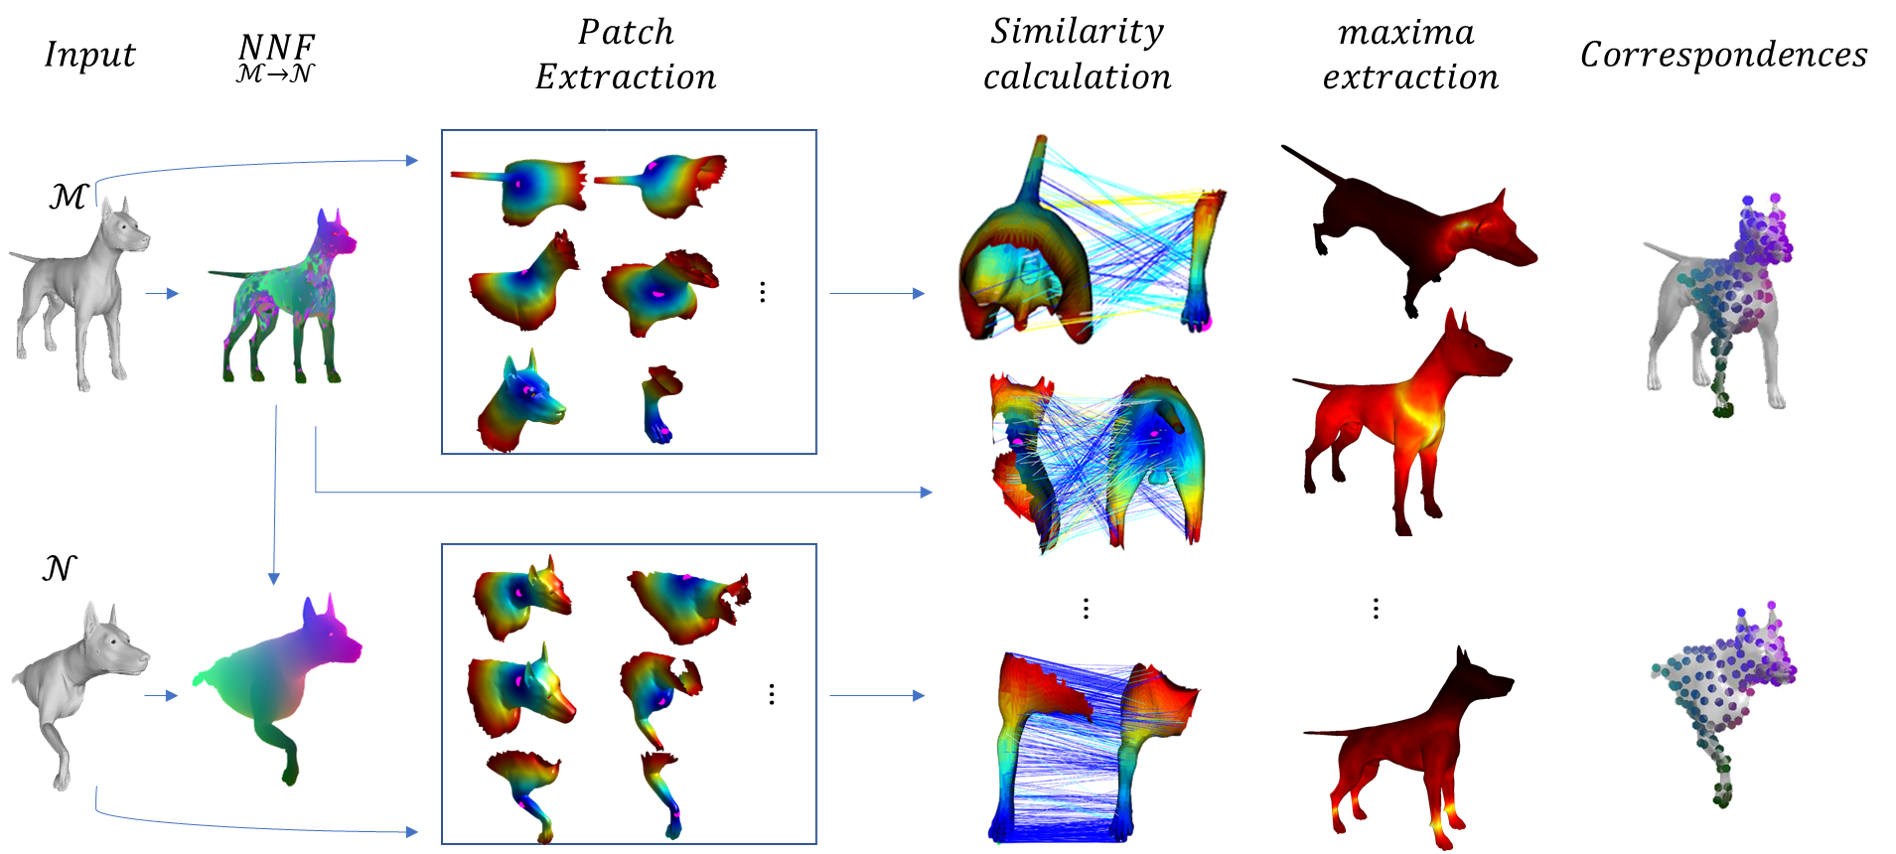
\includegraphics[width=1\textwidth]{figures/Birds_Flight.png}
	\caption{High level illustration of the DDIS Partial Correspondence pipe.}
\end{figure*}

{\color{red}
	
	1. Goal of this section
}
In this section we will describe the application of DDIS framework for matching of partial deformable shapes.

{\color{red}
	2. Key ideas of the algorithm
}
The core of the method lies in utilizing DDIS as a similarity measure between surface parts. While partiality and non rigid deformations causes pointwise descriptors to be inexact, the underlying distribution of the data is still approximately the same for corresponding surface patches.
As in 2D, correct corresponding points between a template and a matching object should lie in nearby regions with relation to some reference point on the template.
However, the preservation of distances holds only approximately even for full template matching, and even less so in the presence of partiality and topological noise.
It holds that the longer a distance between 2 points is, the more likely it is that a distortion had occurred on the geodesic path between them. Thus, instead of using the entire part for a correspondence between 2 points, we use a subset of it for the matching. 
Instead of looking for one central point as done in the original paper, we sample many points and treat each of them as a separate template for matching. Thus obtaining better localization. Even though we do not consider the entire part, and thus do not enforce global coherency, matches stemming from this framework are overwhelmingly correct, and this give way to simple scheme of pruning bad matches.
Finally, we observe that DDIS has different properties at different scales and thus employ a multi-scale cascade to take advantage of this fact.

{\color{red} 	3. Outline of the algorithm (Preprocessing (normal estimation, FPFH), Finding the landmark points, computing DDIS correspondence for pairs, computing correspondence of surfaces)
	Include an image of this general overview.}
\subsection{Algorithm Outline}
We employ the following pipeline to obtain a sparse set of correspondences. We begin by finding extremities on the part $\mathcal{N}$ and use them as anchors for a quasi uniform sampling of the part. We define a template for each of the sampled points by extracting a geodesic disk in a defined radius around it. We calculate point-wise descriptors for both $\mathcal{N},\mathcal{M}$ and the induced nearest neighbor field. We then traverse all the points on $\mathcal{M}$, calculating deformable diversity similarity between it and all the query points and pick the pairs maximizing these as the initial set of correspondences. We then filter out matches which have a high distortion score and use a greedy search for a better match for these from the set of local similarity maximas. 

{\color{red}
	4. Road-map to the section
}
We will begin with a description of the changes made for the deformable diversity framework as a result of moving from 2D to 3D. We will then go over the specific stages of preprocessing necessary for Deformable Diversity in 3D. We will continue with describing the matching process of a single mini template on a full shape. Finally we will describe the extraction of multiple correspondences using this framework.


\subsection{Deformable Diversity Similarity in 3D}
\begin{figure}[htb]
	
	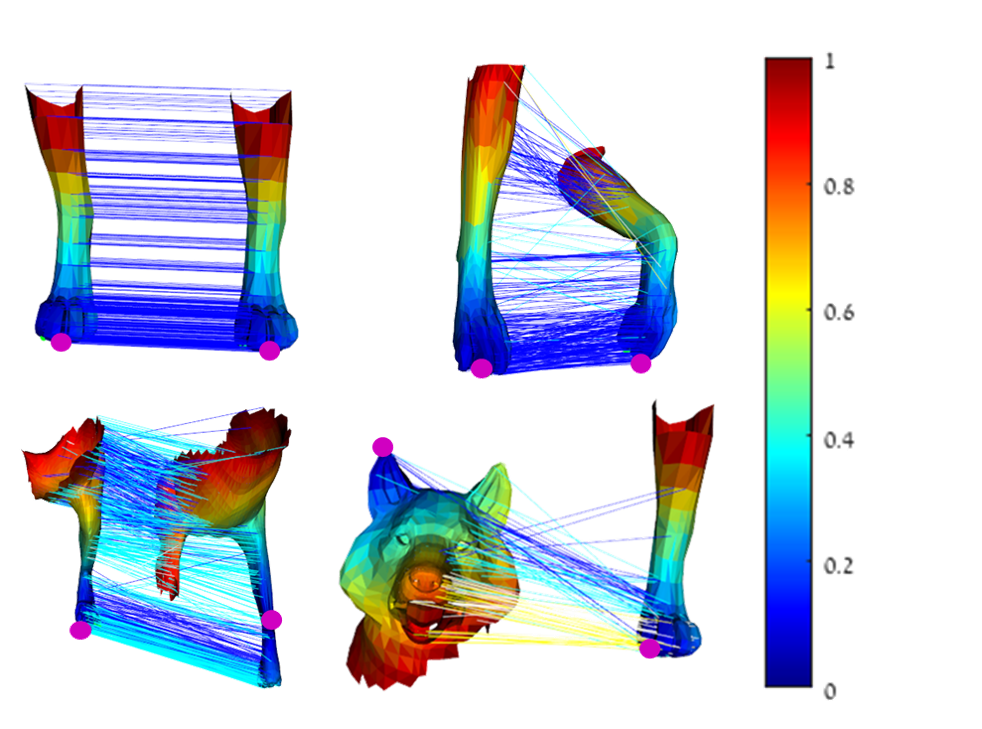
\includegraphics[width=0.5\textwidth]{figures/DDIS2.png}
	\caption{Illustration of Diversity Similarity between different shapes. 
		Geodesic Distances are color coded by the jet scheme. 
		You can notice that on identical pieces, and even on deformed matching pieces there are multiple diverse matches, most of which are colored in blue to indicated very similar distances from the source point, whereas on different pieces most lines map to very few points and a lot of yellow lines (high deformation) exist}
\end{figure}

The nature of 3D data gives rise to unique problems which do not occur in the 2D scenario. Data is distributed in space both sparsely and with varying densities - the amount of data points occupying a given volume can vary drastically.
A second problem arises from the absence of a regular grid. These problems require different definitions for key components to the 2D deformable diversity formulation. For this work we chose the image patch to be replaced by a neighborhood which is required to calculate a selected shape descriptor, usually a small sphere in euclidean space or a surface patch with a radius $r_F$. The search window  of a template is defined as a geodesic disc around the query point, with a radius denoted by $R_T$. The pixel grid distance is replaced by either a euclidean distance $d_{Euc}(x^l,y^l)$(in the case of point clouds) or geodesic distance $d_{Geo}(x^l,y^l)$(for surface meshes).
Given these DDIS  between shape parts $\mathcal{M}_{x,R_T}$ and $\mathcal{N}_{y,R_T}$ can be naively formulated as:
\begin{equation}
DDIS=c\cdot\sum_{m_j\in\mathcal{M}_{x,R_T}}\frac{exp(1-\kappa(NN^S(m_j,\mathcal{N}_{y,R_T}))}{1+r_j}
\end{equation}
where $\mathcal{M}_{x,R_T}$ and $\mathcal{N}_{y,R_T}$ are the shape parts in a radius $R_T$ surrounding the points $x\in \mathcal{M}$ and $y \in \mathcal{N}$ respectively, $r_j$ is the induced deformation
\begin{equation} 
r_j=\frac{|d(m_j^l,m_x^l)-d(NN^S(m_j,\mathcal{N}_{y,R})^l,n_y^l)|}{\gamma\cdot R_T}
\end{equation}
,where $\gamma$ is a selected fraction and $c$ is a normalization coefficient $c=1/min{|\mathcal{N}_{y,R_T}|,|\mathcal{M}_{x,R_T}|}$.

However, we wouldn't like to penalize our similarity score in case of repeating patterns or symmetrical shapes which have both symmetries in the template search window. Intuitively and empirically the exponent is too harsh and indeed unnecessary as both deformity and diversity will attenuate the score in case of multiple nearest neighbors. On the other hand, we wouldn't want to reward far correspondences at all. 
{\color{red} explain why -- can we see it visually on the same example?}{\color{green} no visual example yet, as the partition into smaller templates mitigates some of the problems of the old formulation it seems, though the new one has still given an extra 2 percent of accurate matches even in the mini template setting}\\

To account for this the following formulation has been found to work better: given a point $n_i\subset \mathcal{N}_{y,R}$ has a set of nearest neighbors in descriptor space on a geodesic disc 
$\mathcal{M}_{n_i}=\{m_j\in\mathcal{M}_{j,R_T}:NN^S(m_j,N_{y,R_T})=n_i\}$ 
, we define 
$m_i' = \underset{m_j\in\mathcal{M}_{n_i}}{argmin}\space (r_j)$
and $r_i'$ the minimal distortion distance, we add only the contribution of this point to the similarity score which then becomes
\begin{equation}
DDIS(N_{y,R_T},\mathcal{M}_{x,R_T},\gamma)=\sum_{m_i'}\frac{1}{1+r_i'}
\end{equation}
This equation still promotes both diversity and low deformations, but is less biased toward surfaces which are either symmetrical, or exhibit repeating patterns.

%%%%%%%%%%%%%%%%%%%%%%%%%%%%%%%%%%%%%%%%%%%%%%%%%%%%%%%%%%%%%%%%%%%%%%%
%%%%%%%%%%%%%%%%%%%%%%%%%%%%%%%% section: DDIS Correspondence between a Point and a Surface
%%%%%%%%%%%%%%%%%%%%%%%%%%%%%%%%%%%%%%%%%%%%%%%%%%%%%%%%%%%%%%%%%%%%%%%
\subsection{DDIS Template Matching}
{\color{red} Goal of the algorithm}
In this section we go over the flow of template matching of 3D shapes using DDIS, the solution of which constitutes the core of our partial shape matching. Given a template $\mathcal{N}_{y,R_T}$ with a reference point $n_y$ as it's center and a maximal distance $R_T$, we aim to find on a model $\mathcal{M}$ which has a deformed version of it, the corresponding surface piece $\mathcal{M}_{y*,R_T}$ and it's center $m_y*$. The solution is obtained by finding the point on $\mathcal{M}$ whose surrounding geodesic disc maximizes the above mentioned DDIS measure.
{\color{red}key ideas}

{\color{red} Overview}
We'll first give an overview, and then give an extended description of each of each stage. 

We start by calculating the normals for $\mathcal{M}$ and $\mathcal{N}$.
We than calculate local point descriptors for each patch of some neighborhood around the points in each mesh(For our purpose FPFH seemed to work the best of our tested descriptors). 
Having calculated these, we calculate a nearest neighbor field by finding for each patch in $\mathcal{M}$ it's Nearest Neighbor in $\mathcal{N}$. 
We now find the distance of every point $n\in \mathcal{N}$ to the desired point $y\in \mathcal{N}$ for a desired neighborhood $R_T$.
We now go over every point $x\in mathcal{M}$. For each we extract the geodesic disc $\mathcal{M}_{x,R_T}$ around it.
We take notice that while the above stages are done here in the context of template matching for one template, when matching multiple templates all of the above calculations have to be done only once between the shapes, with the exception of geodesic distance field extraction for the template itself. 
Finally we calculate DDIS for this disc with $\mathcal{N}_{y,R}$ which has $y$ as it's center. Having done that for every point, the point $y*\in \mathcal{M}$  which gets the maximal DDIS Score is deemed the corresponding point to $y$.


\textbf{Point Normal Estimation}
There are various schemes for estimating point normals given a triangulated mesh surface. We have picked the one which is available in the standard PCL. Given a vertex $p_i$ on a triangulated mesh $\mathcal{X}$ and it's associated polygons $\{A_j\}_{j=1}^k$ and their normals $N_{A_j}$ the point normal $N_i = \sum_{j=1}^k{|A_j|\cdot N_{A_j}}$

\textbf{Local Patch Size choice}
DDIS as defined by \cite{talmi2017template} uses patch descriptors as low level features for their similarity measure. While a patch in an image can by defined by the images grid no such grid exists on 3D point clouds and meshes, where density of data points can vary. Thus a patch has to be defined by some geometric measure. While the more robust way to define it would be using geodesic distance, since we are talking a small environment around a point on the mesh we have found that for practical purposes a patch in a defined euclidean radius $r_F$ around a point serves well enough. We pick this radius in the following way: given the full surface mesh $\mathcal{M}$ we find it's equivalent of a diameter $D_\mathcal{M} = \sqrt{Area(\mathcal{M})}$, and tune a parameter $\alpha$ to obtain $r_{F} = \frac{\alpha}*D_\mathcal{M}$

\textbf{Local Patch Descriptor}
A lot of local shape descriptors have been used successfully in 3D shape analysis. We have tested the following descriptors: PFH\cite{rusu2008learning} SHOT\cite{tombari2010unique},HKS\cite{Sun:2009:CPI:1735603.1735621},SIHKS\cite{bronstein2010scale},ROPS\cite{guo2013rotational} and FPFH\cite{rusu2009fast}. Out of these FPFH has achieved the best performance, and thus the descriptor for the local patch has been chosen to be FPFH. 

\textbf{Nearest Neighbor Field}
As an intermediate stage towards the calculation of Deformable Diversity Similarity measure, the calculation of the nearest neighbor field(will be abbreviated as $NNF$) needs to be calculated. Thus for every patch $m\in \mathcal{M}$ we have to find the patch on the template $n\in\mathcal{n}$ which resembles it the most. For $FPFH, NN^S(m_j,\mathcal{N})$ is defined $NN^S (m_j,\mathcal{N}) \equiv \underset{i}{argmin}\chi^2(FPFH(m_j],FPFH(n_i))$ and the Nearest Neighbor Field is the set of all these correspondences.

\textbf{DDIS calculation}
For every point in $m_x\in\mathcal{M}$ we then extract a geodesic disk $\mathcal{M}_{x,R}$ with a radius $R_T$ around it and calculate deformable diversity score for it. The point which maximizes the similarity score gives us a correspondence $(y,y*)\in \mathcal{N}\times\mathcal{M}$.
%\\Since as we will show in the results section, imperfections in the isometry assumption lead to considerable localization errors, we move to a multiple template matching framework using DDIS, as will be described in the next section. 

%%%%%%%%%%%%%%%%%%%%%%%%%%%%%%%%%%%%%%%%%%%%%%%%%%%%%%%%%%%%%%%%%%
%%%%%%%%%%%%% section: DDIS Sparse Correspondence
%%%%%%%%%%%%%%%%%%%%%%%%%%%%%%%%%%%%%%%%%%%%%%%%%%%%%%%%%%%%%%%%%%
\subsection{DDIS Sparse Correspondences}
A key takeaway from experimenting with DDIS as a template matching algorithm for partial matching has been that isometry does not hold, at least not globally.It does however, hold pretty well locally, especially at extremities. To this end we devise  multiple template matching framework for Partial correspondences of deformable shapes. We first obtain landmarks $F_init=\{f\}_i$ as described in[]. 
We then employ a simple sampling scheme which ensures a good quasi uniform covering of the surface.
Finally, we for each sample point we extract a geodesic disc, and find its counterpart on $\mathcal{M}$ which maximizes DDIS. 

\textbf{Landmark Extraction}
We follow the work of [Sagi Katz Ayellet Tal] to obtain interesting landmark points. Given a shape the work employs the following framework to extract it's extremities. A point is detected as an extremity if it fulfills 2 conditions: - it's sum of geodesic distances is a local extrema, formally, for $v\in S$ ,where $S$ is a surface mesh, we define the set of points with a direct edge to it as $N_v$, the point is a critical point if :
\begin{equation}
\sum_{v_i\in S}d_{geo}(v,v_i)>\sum_{v_i\in S}d_{geo}(v_n,v_i), \forall v_n\in N_v
\end{equation}
An additional requirement for it to be an extremities is for it to lie on the convex hull of the shape's MDS. In this work we have dropped the last condition, but chose $N_v*$ - a neighborhood of $0.03\cdot \sqrt{Area(S)}$.

%%%%%%%%%%%%%%%%%%%%%%%%%%%%%%%%%%%%%%%%%%%%%%%%%%%%%%%%%%%%%%%%%%
%%%%%%%%%%%%% subsection: Landmark Template Matching
%%%%%%%%%%%%%%%%%%%%%%%%%%%%%%%%%%%%%%%%%%%%%%%%%%%%%%%%%%%%%%%%%%

\begin{algorithm}[h]
	\caption{3DIS Sparse Correspondences}
	\begin{algorithmic}
		\Procedure{DDIS Correspondence}{$\mathcal{M},\mathcal{N},\alpha,\beta,\gamma$}\Comment{Returns point correspondence for critical points on $\mathcal{N}$}
		\State{$r_F\leftarrow \alpha /100 \cdot \sqrt{Area(\mathcal{M})}$}
		\State{$R_{thresh}\leftarrow \beta /100 \cdot \sqrt{Area(\mathcal{M})}$}
		\State{$N_\mathcal{M}\leftarrow ComputeNormals(\mathcal{M})$}
		\State{$N_\mathcal{N}\leftarrow ComputeNormals(\mathcal{N})$}
		\State{$F_\mathcal{M}\leftarrow FPFH(\mathcal{M},N_\mathcal{M},r_F)$}
		\State{$F_\mathcal{N}\leftarrow FPFH(\mathcal{N},N_\mathcal{N},r_F)$}
		\State{$NNF_{\mathcal{M}\rightarrow \mathcal{N}}\leftarrow ANN(F_\mathcal{M},F_\mathcal{N})$}
		\State{$\mathcal{N}_c=\{n:\sum_{n_i\in\mathcal{N}}d_{geo}(n,n_i) > \sum_{n_i\in\mathcal{N}}d_{geo}(n_N,n_i), \forall n_N:d_{geo}(n,n_N)<0.03\cdot \sqrt{Area(\mathcal{M})}\}$}
		\For{$n_y\in \mathcal{N}_c$} \Comment{DDIS calculation Loop}
		\State{$m_c*\leftarrow DDIS\_Correspondence(\mathcal{M},n_y,\mathcal{N},\alpha,\beta,\gamma)$} 
		\EndFor
		\State{return $\mathcal{M}_c\times\mathcal{N}_c=
			\{m_c*,n_c\}$}
		\EndProcedure
	\end{algorithmic}
\end{algorithm}

\textbf{Landmark Template Matching}
For this end, we create a template for each landmark point - we collect all surface point in a geodesic neighborhood around it of $\beta\cdot\sqrt{area(\mathcal{M}}$  where for this case a good $\beta~(0.2,0.5)$ where larger $beta$ prevents global scale error, such as a cats paw being mapped to a hind paw, while smaller beta promotes tighter localization on the part itself. This can be seen in Figure[] While it might seem natural to calculate a different nearest neighbor field for each landmark template it has been empirically found that using the global nearest neighbor field gives much better results. This is probably due to the fact that the nearest neighbor field encodes global information when obtained this way and eliminates local distractors.
Each landmark template is compared to all surface parts of a similar $R$ on $\mathcal{M}$ to obtain final point correspondences.


%%%%%%%%%%%%%%%%%%%%%%%%%%%%%%%%%%%%%%%%%%%%%%%%%%%%%%%%%%%%%%%%%%
%%%%%%%%%%%%% section: Multi-Scale DDIS
%%%%%%%%%%%%%%%%%%%%%%%%%%%%%%%%%%%%%%%%%%%%%%%%%%%%%%%%%%%%%%%%%%
\subsection{Cascaded Multi-Scale DDIS}
The observation of the effects of the choice of $\beta$ and the trade-off between finer localization and avoidance of global errors naturally leads to the adoption of a multi scale framework. We calculate $DDIS$ score for multiple $beta$ values, and use the location obtained with a large beta to select a narrow environment in which we look for the maximum of DDIS with a smaller value $beta$, thus using the larger scale to get a rough global location, and the smaller scale to fit it into a more exact location. While this might be done at multiple custom scales we have found that the triplet $\beta ,2\cdot beta/3\beta/3$ works well.
\begin{figure}[htb]
	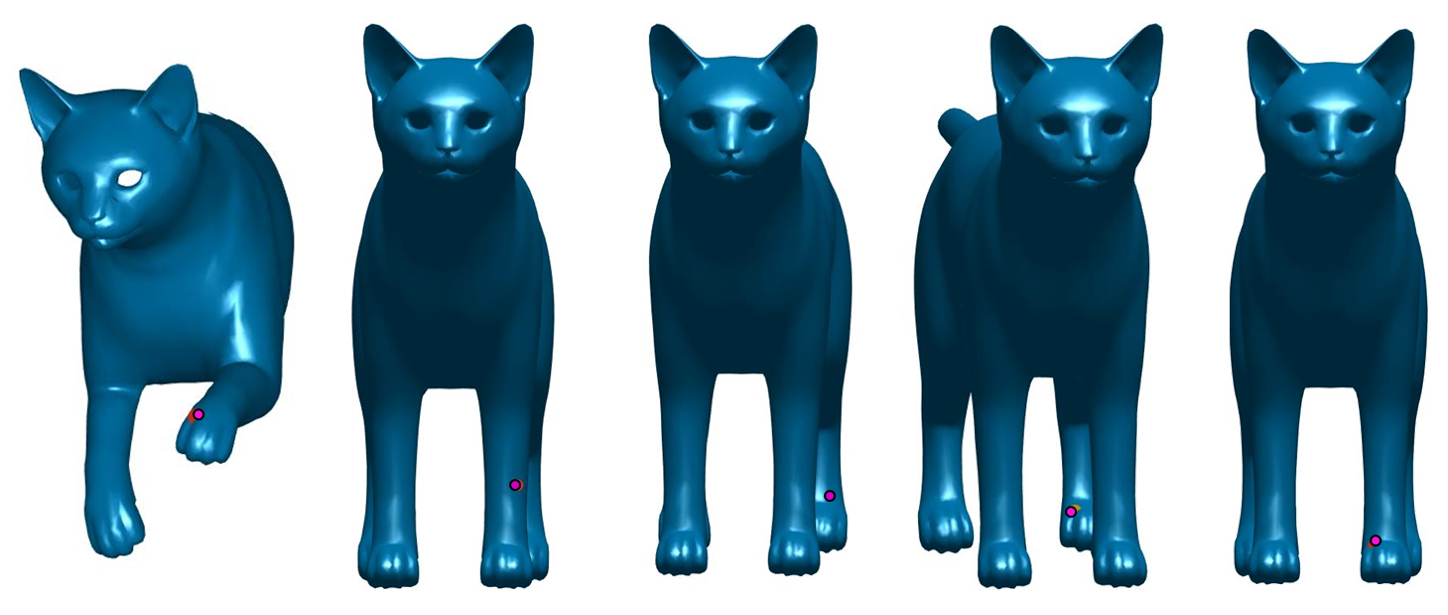
\includegraphics[width=0.5\textwidth]{figures/MultiScaleDis.png}
	\caption{Illustration of the multi scale framework. Gray point are the area chosen by the previous scale to be valid. It can be seen that Wrong maxima in lower scales are ignored due to this process}
\end{figure}

\begin{figure*}
	\centering
	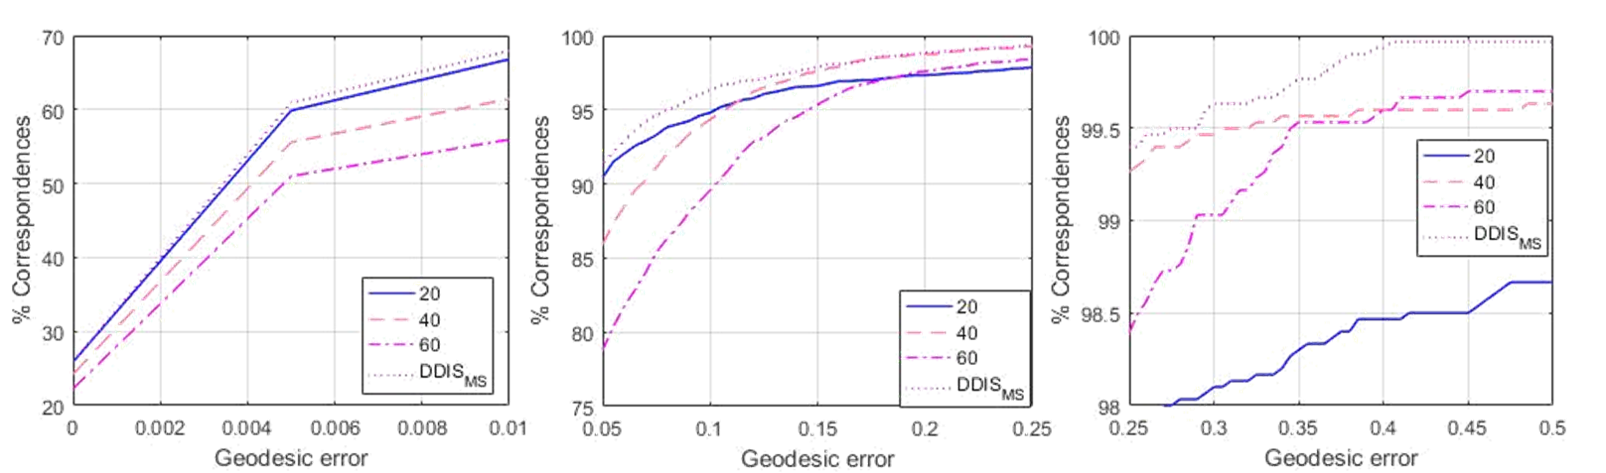
\includegraphics[width=1\textwidth]{figures/AblationStudyThreshold.png}
	\caption{Effect of the $\beta$ parameter on the results: it can be seen that a smaller beta promotes better localization in a small neighborhood, while higher values of $\beta$ lead to more local errors but are more robust to global errors. It can be seen that the multi-scale cascade achieves better results both locally and globally.}
\end{figure*}
\section{Experiments and results}\label{section:results}

In this section we will briefly go over the experiments performed and their results. We'll introduce the datasets, detail our experiments and their results
\subsection{Datasets}
In this section we will briefly go over the available Datasets
\subsubsection{SHREC 2016}  
The SHREC partial matching dataset consists of 8 base, neutral pose models: cat, centaur, dog, horse, wolf, and 3 humans – 2 males, and 1 female. Each basic model has corresponding deformed partial shapes obtained either by cutting the shape with a plane or by adding holes on a deformed shape. The set has been divided into train and test sets. The train set is composed of 15 cuts for each base models totaling 120 models,and 10 holed shpaes for each model for which ground truth point to polygon correspondences has been provided in barycentric coordinates. The test set is composed of additional 200 cuts and 200 holed shapes.


\subsection{Error Metrics}
The output of partial matching algorithms (as defined in\cite{cosmo2016shrec}) are sub-vertex point-to-point correspondences between partial shapes.
For all experiments we use the standard practice of not penalizing symmetric solutions. Quality is measured according to the Princeton benchmark protocol \cite{kim2011blended}. For a pair of points $(x,y)\in \mathcal{N}\times \mathcal{M}$ between the full object $\mathcal{M}$ and the partial shape $\mathcal{N}$ produced by an algorithm, where $(x,y^*)$ is the ground truth correspondence the inaccuracy is measured by 
\begin{equation}
\varepsilon(x)=\frac{d_{\mathcal{M}}(y,y^*)}{\sqrt{area(\mathcal{M})}}
\end{equation}
where $d_{\mathcal{M}}(y,y^*)$ is the geodesic distance on $\mathcal{M}$, and has units of normalized length on $\mathcal{M}$. For dense correspondences over a dataset, $\varepsilon(x)$ is averaged over all matching instances.
\subsubsection{Central Points Localization}
In this experiment we have chosen for each Template mesh the center point $c_T$ and tried to match it to a point on the object using DDIS. Experiments have been done using FPFH, PFH and SHOT as patch descriptors with patch radiuses of $[2,3,4,5]$, the results of the opimal parameter for each descriptor are illustrated in fig. and visualizations of similarity maps of cuts are provided in fig. . It can be seen that good localization is obtained for points on a smooth surface, under high partiality conditions and strong deformations. Bad matches occur when a matched point resides on a heavily deformed patch, and when salient anchor points are deformed or cut.  Analysis of these results shows a drift in localization occurs when salient features are divided by strong unisometric deformations which serve as the motivation for the multiple template matching framework.

\begin{figure*}[htb]
	\centering

	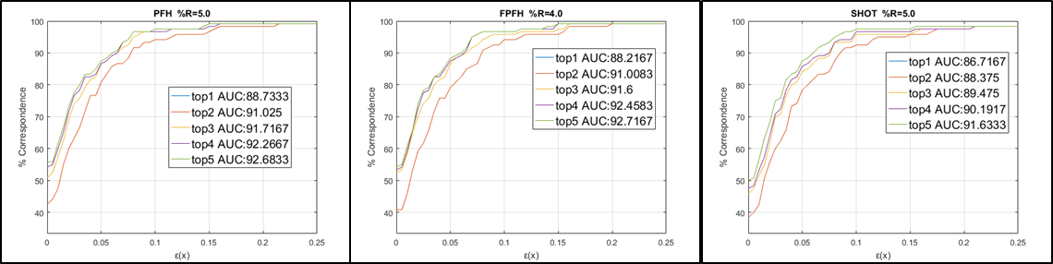
\includegraphics[width=1\textwidth]{figures/ROCfigure.png}
	\caption{Comparison between descriptors: we show curves for the minimal distance of the top results. a noticeable addition occurs when adding the 2nd best match}
\end{figure*}

\subsection{Sparse Correspondences on the SHREC16 Test set}
In this experiment we have tested the performance of DDIS in producing sparse correspondences on the SHREC16 Partial Matching of Deformable Shapes competition. 
We had tuned our parameters on the SHREC16 training dataset using only the cuts part of it. The best results had been produced using FPFH with $r_F = 0.04\sqrt{Area(\mathcal{M}}$, and a piece size radius $R_thresh=0.3\sqrt{Area(\mathcal{M})}$. For Geodesic distances we have found the fast marching algorithm to work the fastest, while giving the lowest error w.r.t. to exact geodesics. For a 10,000 vertices mesh it takes 60s to produce a full distance matrix, Though it should be noted this algorithm has a more efficient GPU implementation. FPFH and Nearest Neighbor field takes 2 s' and similarity between 2 pieces of ~10000 vertices each takes 25s on average, running on a single thread of i7-2700k. Unlike optimization based algorithms this is highly parallelizable.
We achieve results comparable to the state of the art \cite{litany2017fully} quality wise, even though sparser in nature on both the Cuts and the Holes datasets, Where a particularly impressive result is reported on the Holes dataset. A further look reveals even more reliable results can be obtained taking only the extremity points not lying on the mesh longest boundary, but they will be more sparse

\begin{figure*}[htb]
	\centering

	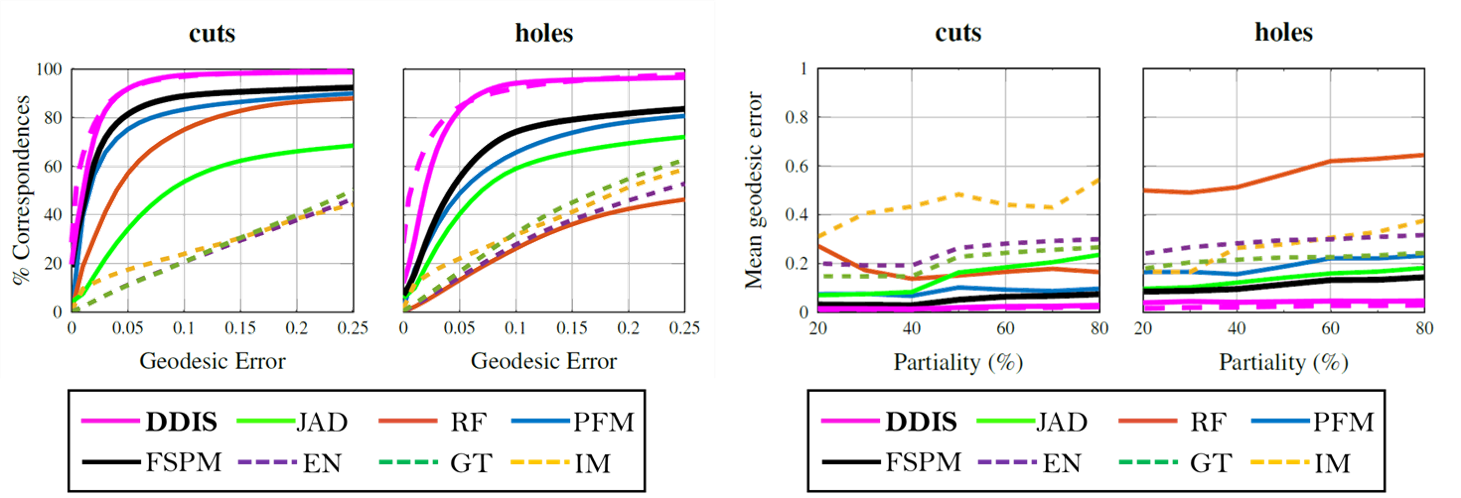
\includegraphics[width=1\textwidth]{figures/ROCSHREC16.png}
	\caption{comparison with other state of the art algorithms - it can be seen that although sparse in nature, the correspondence obtained by DDIS are much more accurate than the other methods. 
		A separate analysis has been done for correspondences which include boundary points, which tend to be more noisy, and internal points which are more sparse}
\end{figure*}

\begin{table}[h]
	\centering
	\begin{tabular}{c  c  c  c  c  c  c c} 
		\hline
		& PFM & RF & IM & EN & GT & DIS & DISnoBound \\ \hline
		cuts & dense & dense & 61.3 & 87.8 & 51.0 & 27.9 & 14.5\\ \hline
		holes & dense & dense & 78.2 & 112.6 & 76.4 & 77.3 & 52.11 \\ \hline
		
	\end{tabular}
	\caption{mean number of correspondence obtained by the algorithms in the SHREC 16 competiton and our algorithm}
	\label{table:1}
\end{table}

\begin{figure*}[htb]
	\centering
	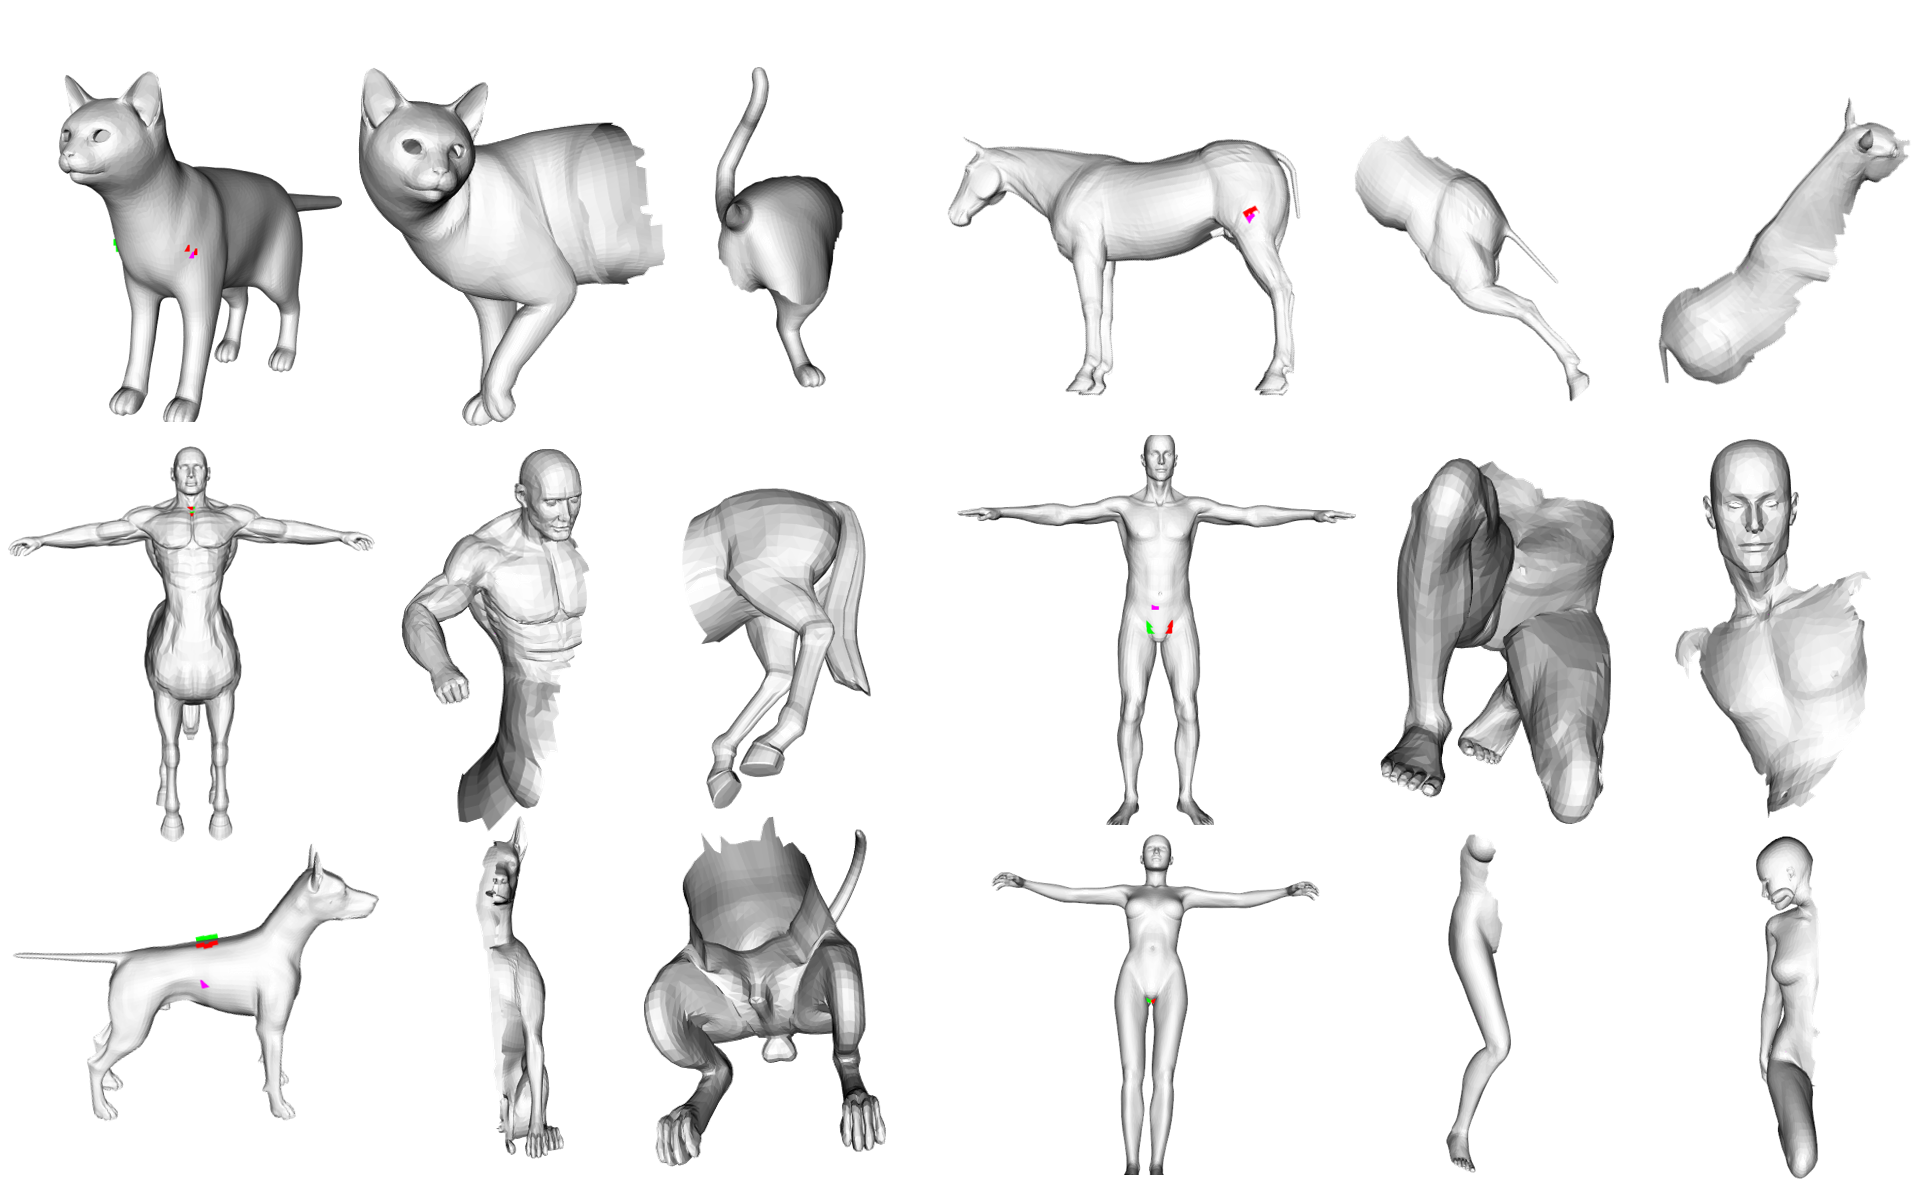
\includegraphics[width=1\textwidth]{figures/Partial_matching_shrec.png}

	\caption{SHREC 16 cuts partial matching dataset.}
\end{figure*}
\begin{figure*}[htb]
	\centering
	\ifpdf
	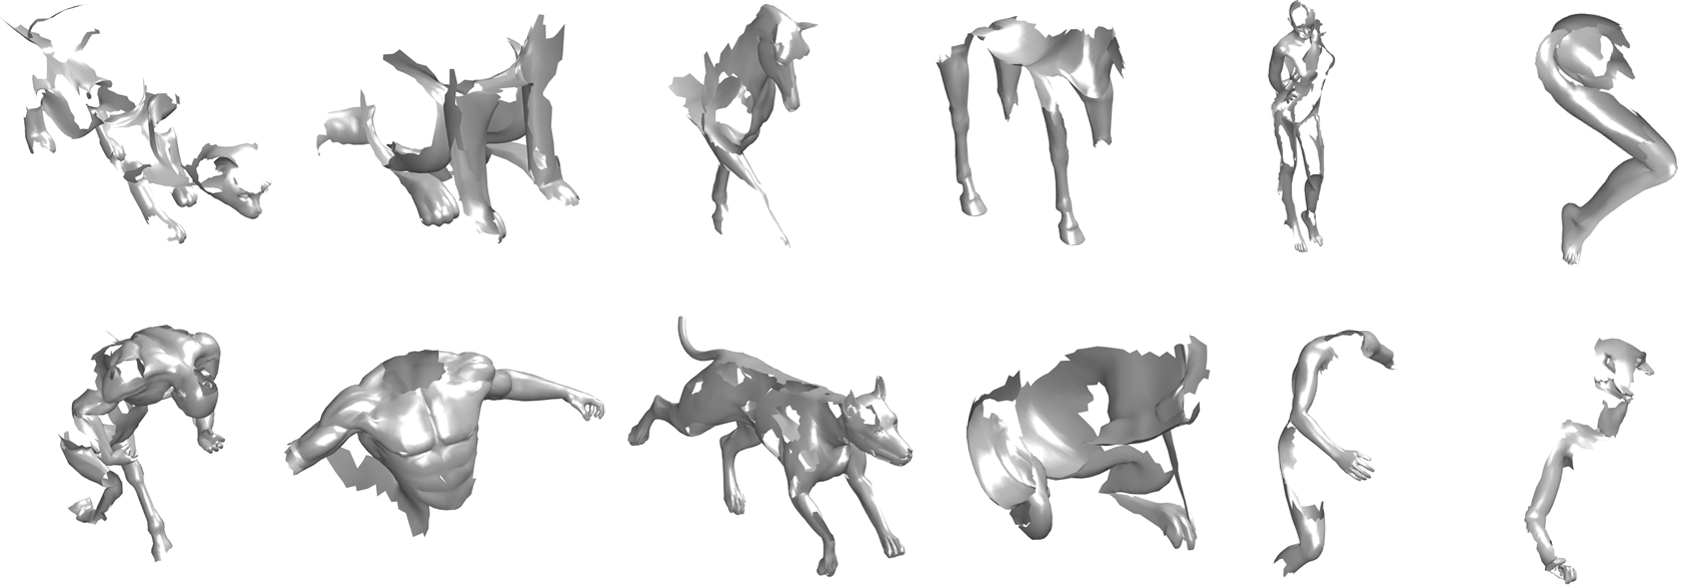
\includegraphics[width=1\textwidth]{figures/Holes.png}
	\else
	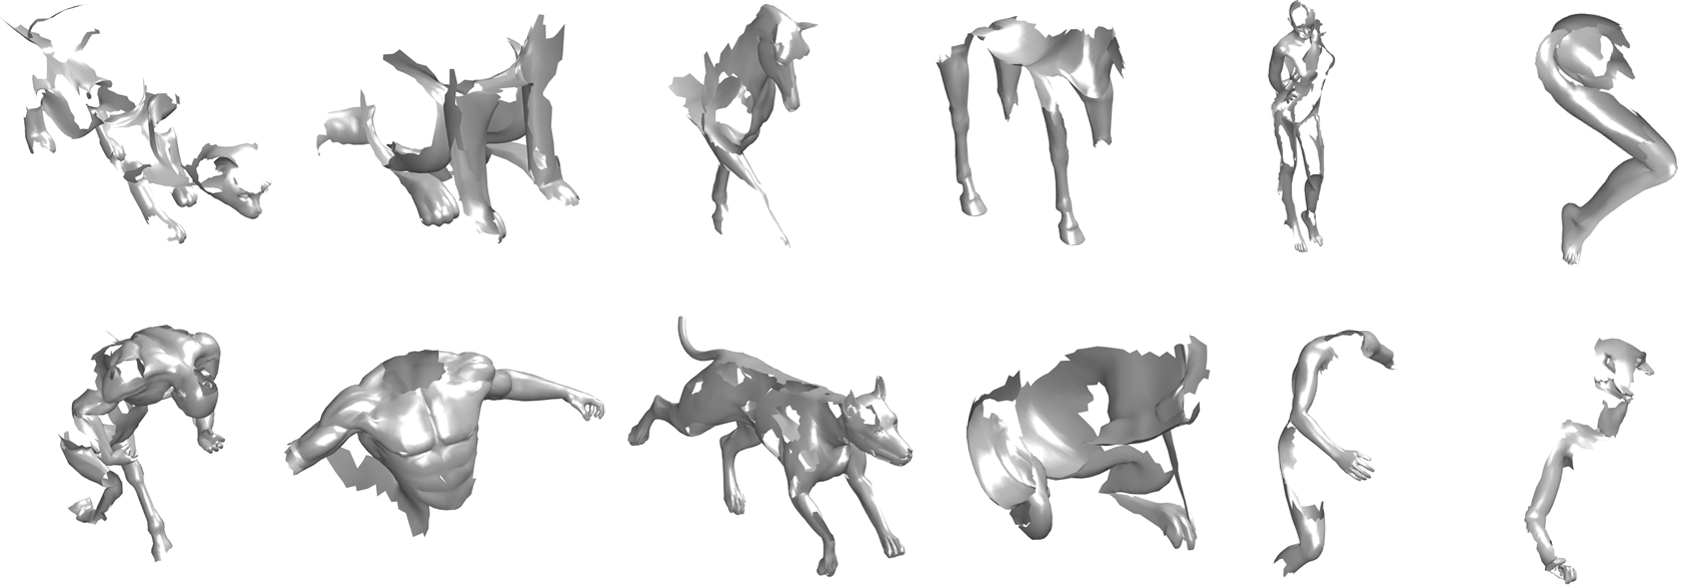
\includegraphics[width=1\textwidth]{figures/Holes.png}
	\fi
	\caption{SHREC 16 holes partial matching dataset.}
\end{figure*}

\begin{figure*}[htb]
	\centering
	\ifpdf
	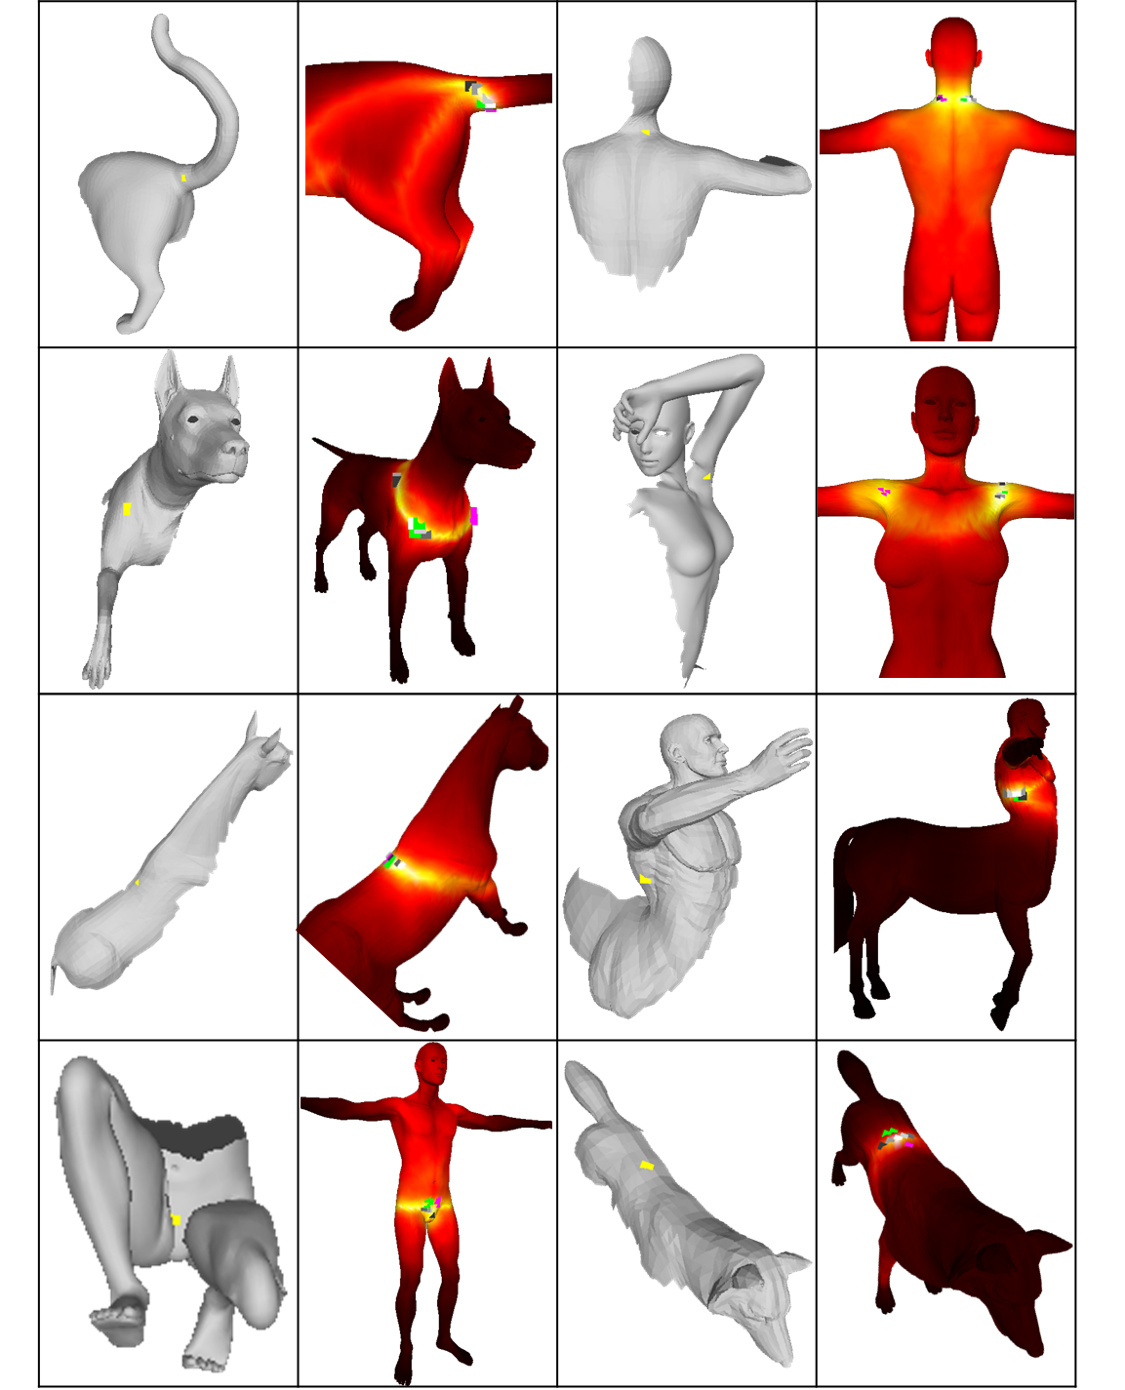
\includegraphics[width=1\textwidth]{figures/success.png}
	\else
	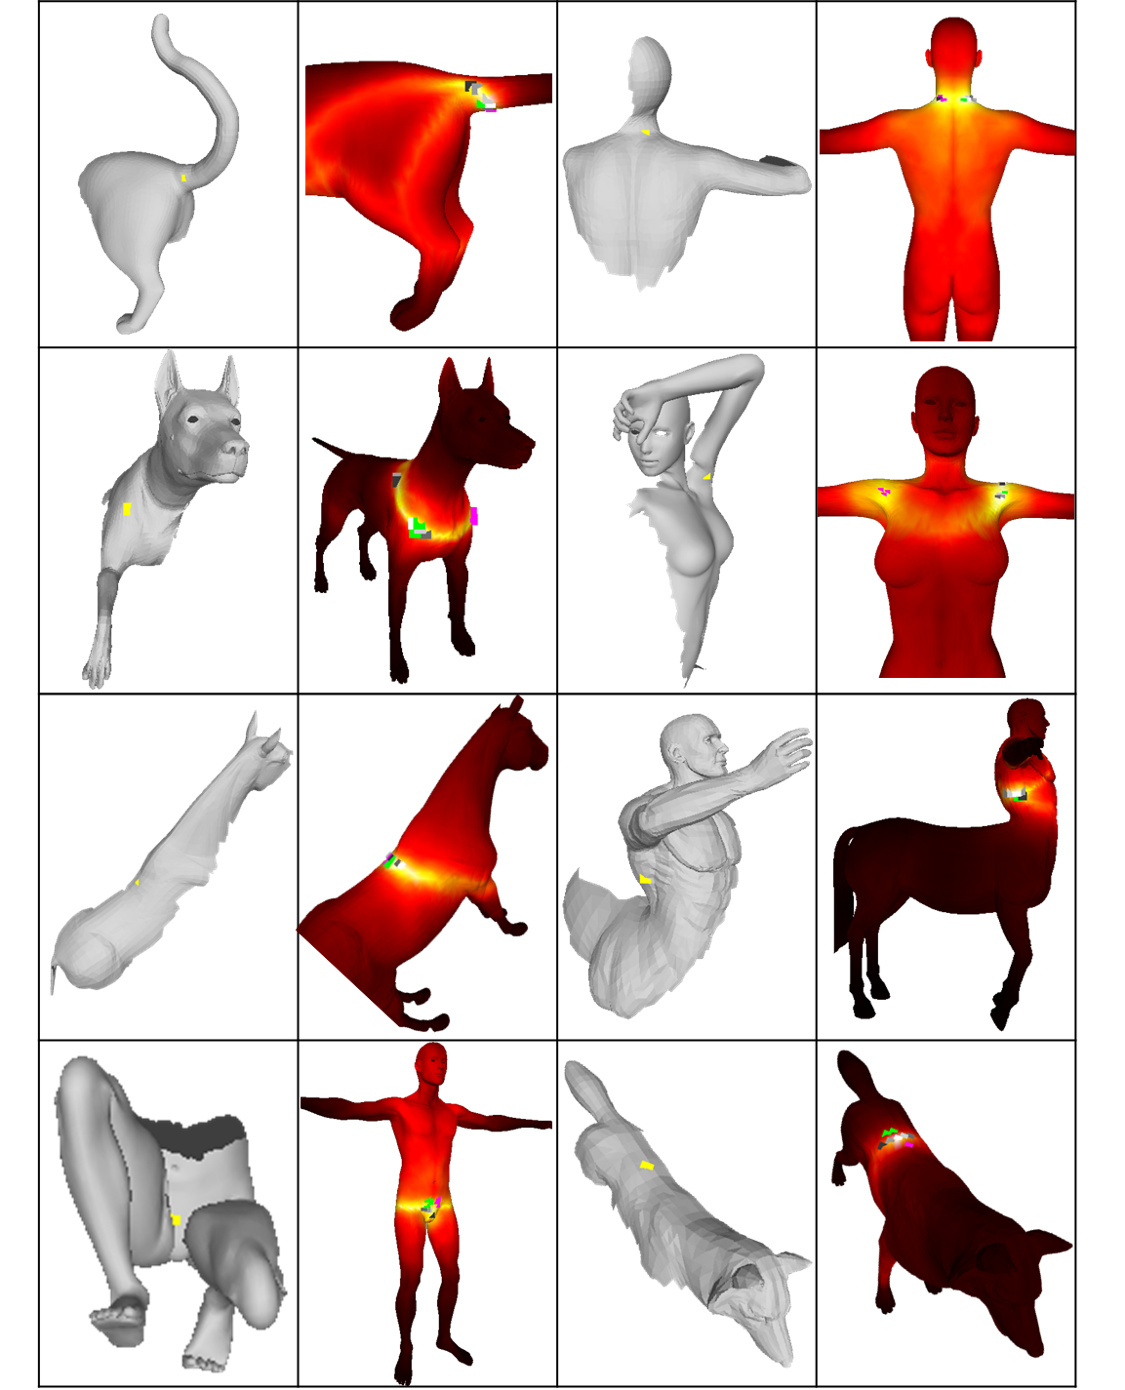
\includegraphics[width=1\textwidth]{figures/success.png}
	\fi
	\caption{Some examples of cuts and their matching similarity score maps. The compared point is marked in yellow on the cut, whereas ground truth polygon is marked in green, symmetrical polygon in purple, and top 5 matches in grayscale}
\end{figure*}

\begin{figure*}[htb]
	\centering
	\ifpdf
	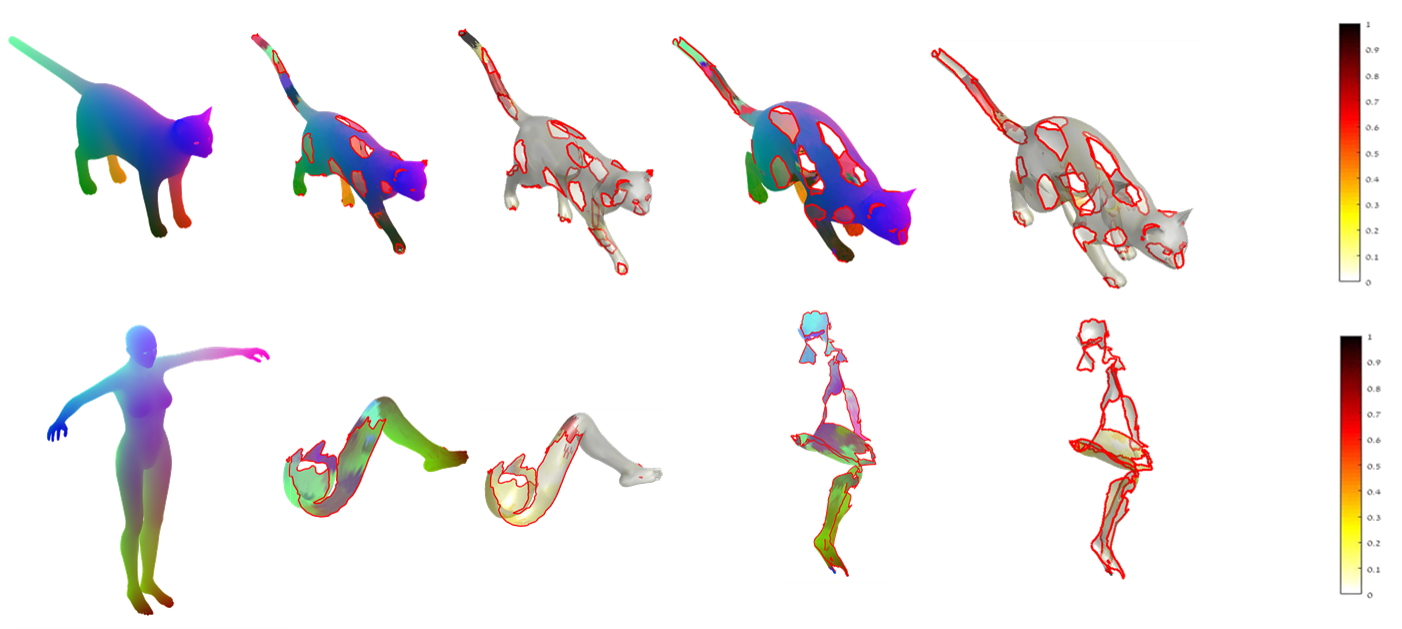
\includegraphics[width=1\textwidth]{figures/failures.png}
	\else
	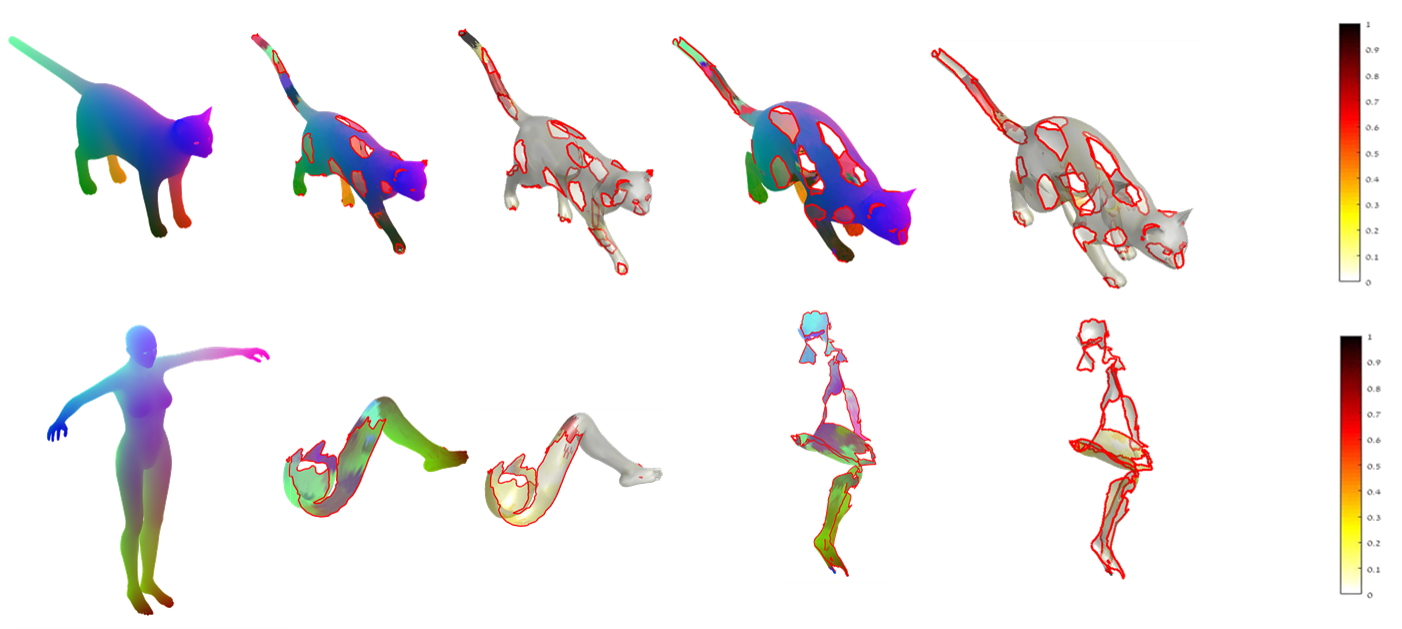
\includegraphics[width=1\textwidth]{figures/failures.png}
	\fi
	\caption{Some notable failure cases: (1)The man's abdomen is unisometrically deformed (2)The cats  }
\end{figure*}
{\small
\bibliographystyle{ieee}
\bibliography{egbib}
}

\begin{figure*}[htb]
	\centering
	\ifpdf
	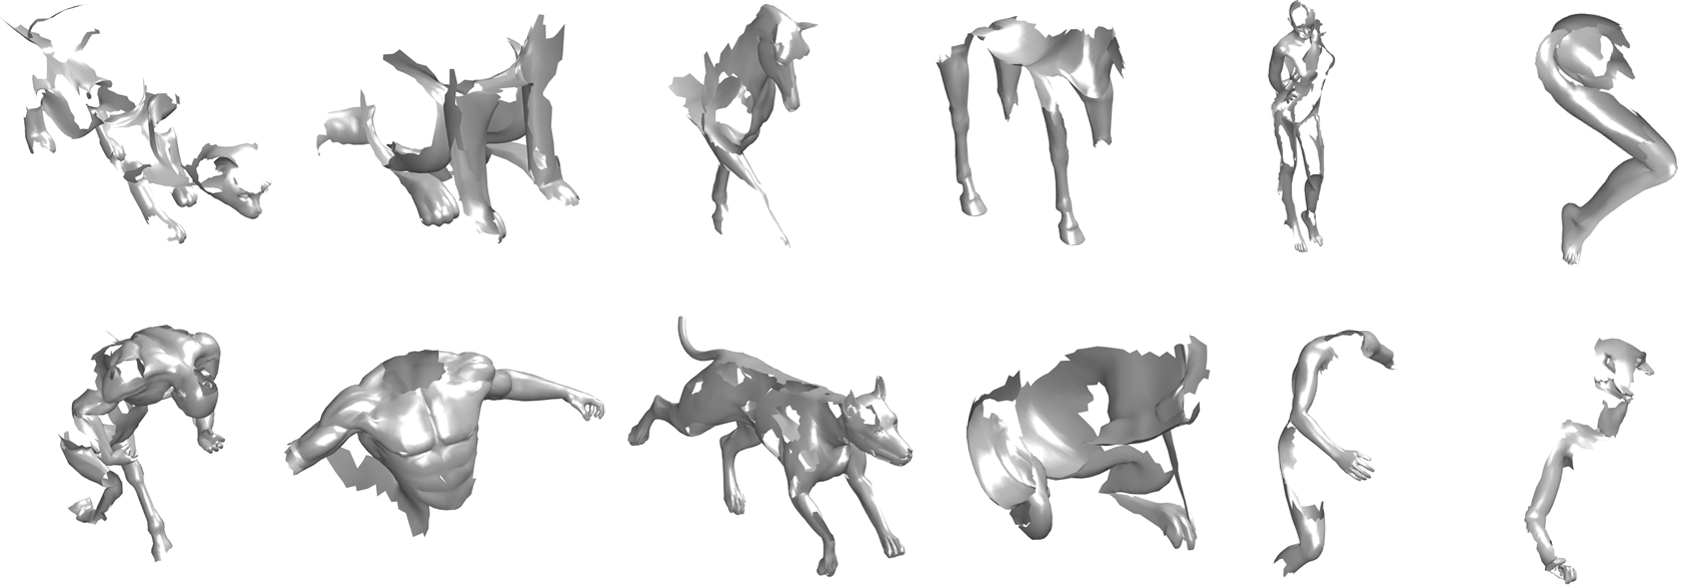
\includegraphics[width=1\textwidth]{figures/Holes.png}
	\else
	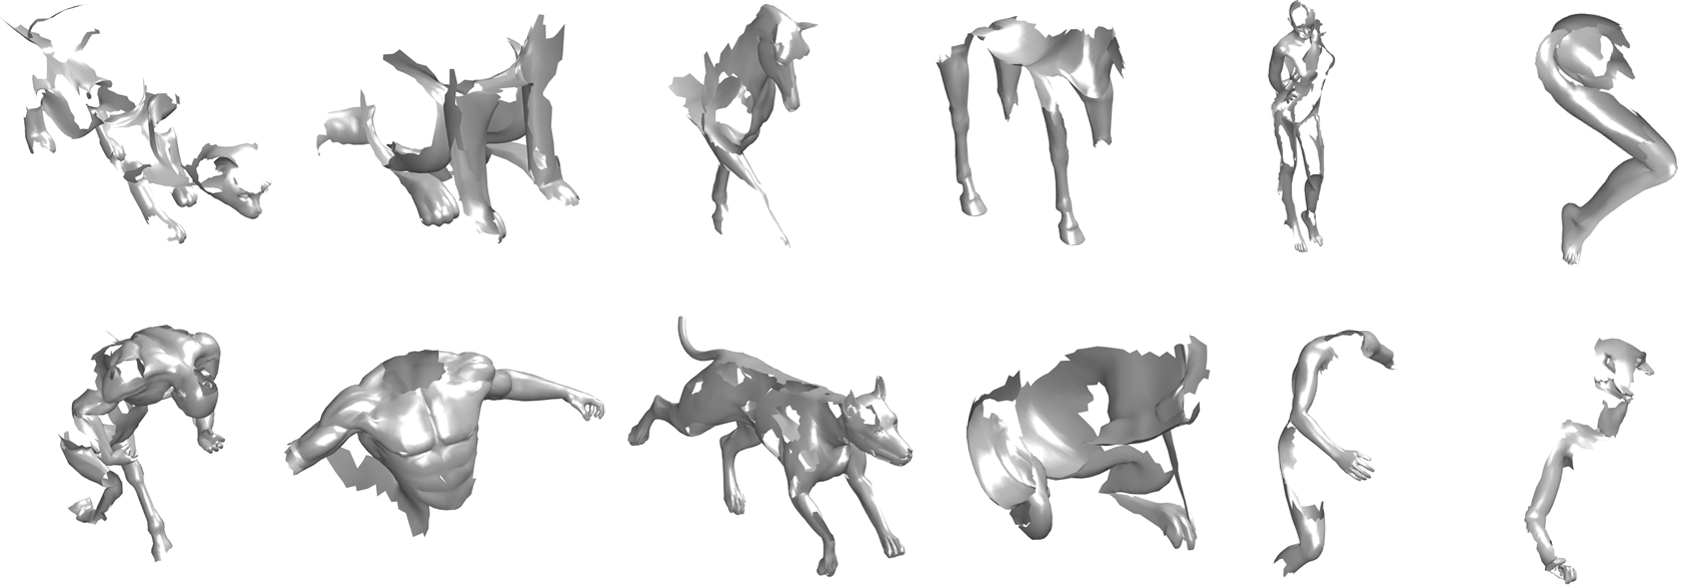
\includegraphics[width=1\textwidth]{figures/Holes.png}
	\fi
	\caption{SHREC 16 holes partial matching dataset.}
\end{figure*}

\begin{figure*}[htb]
	\centering

	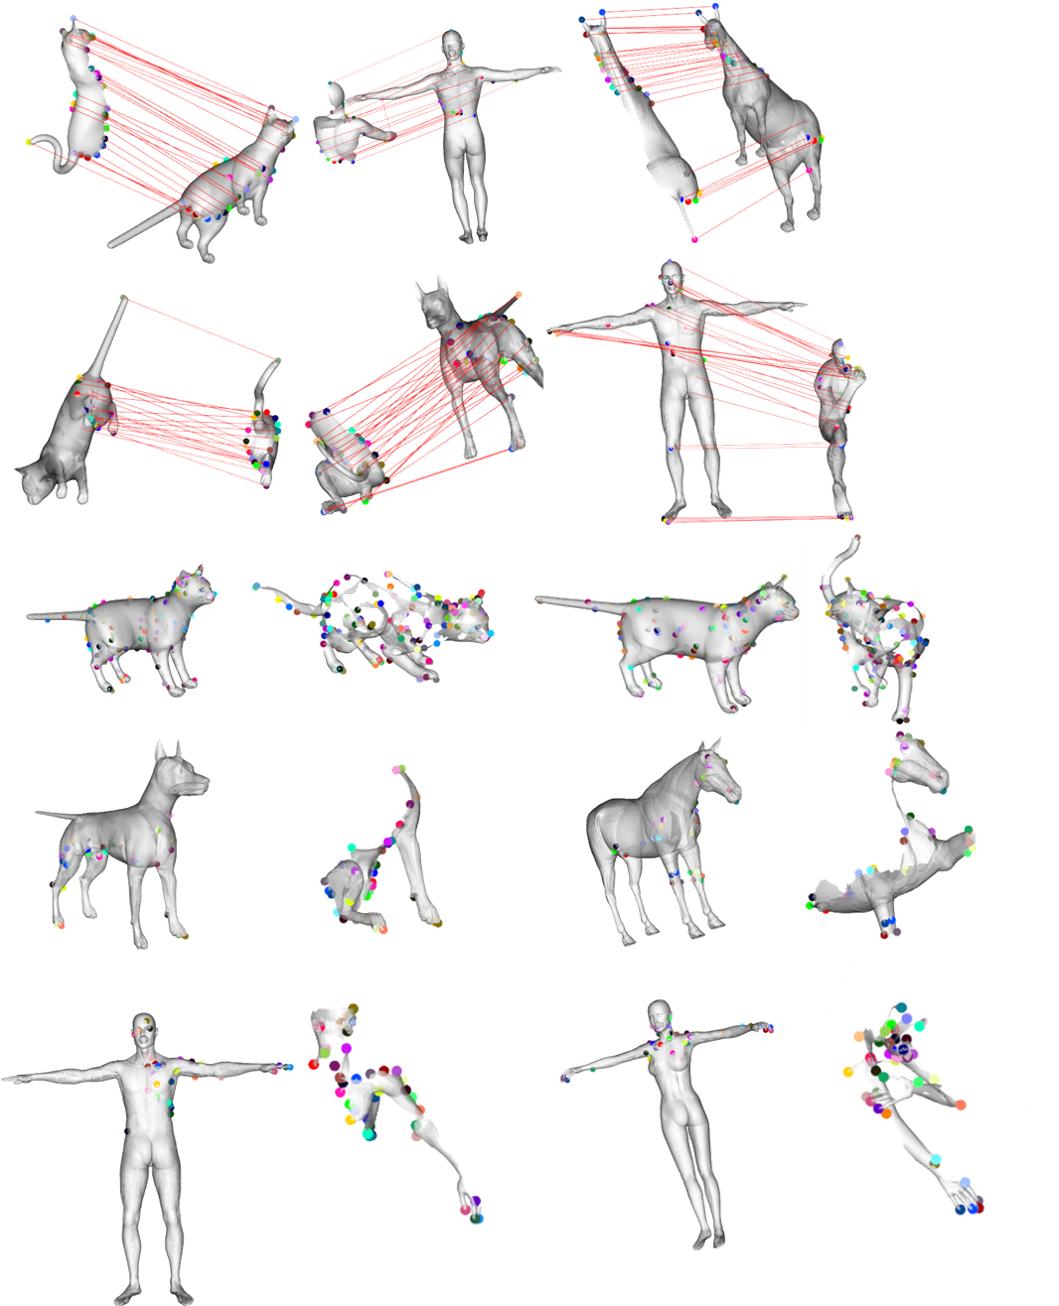
\includegraphics[width=1\textwidth]{figures/success_1}
	\caption{Good correspondences obtained by our DDIS measure}
\end{figure*}

\begin{figure*}[htb]
	\centering
	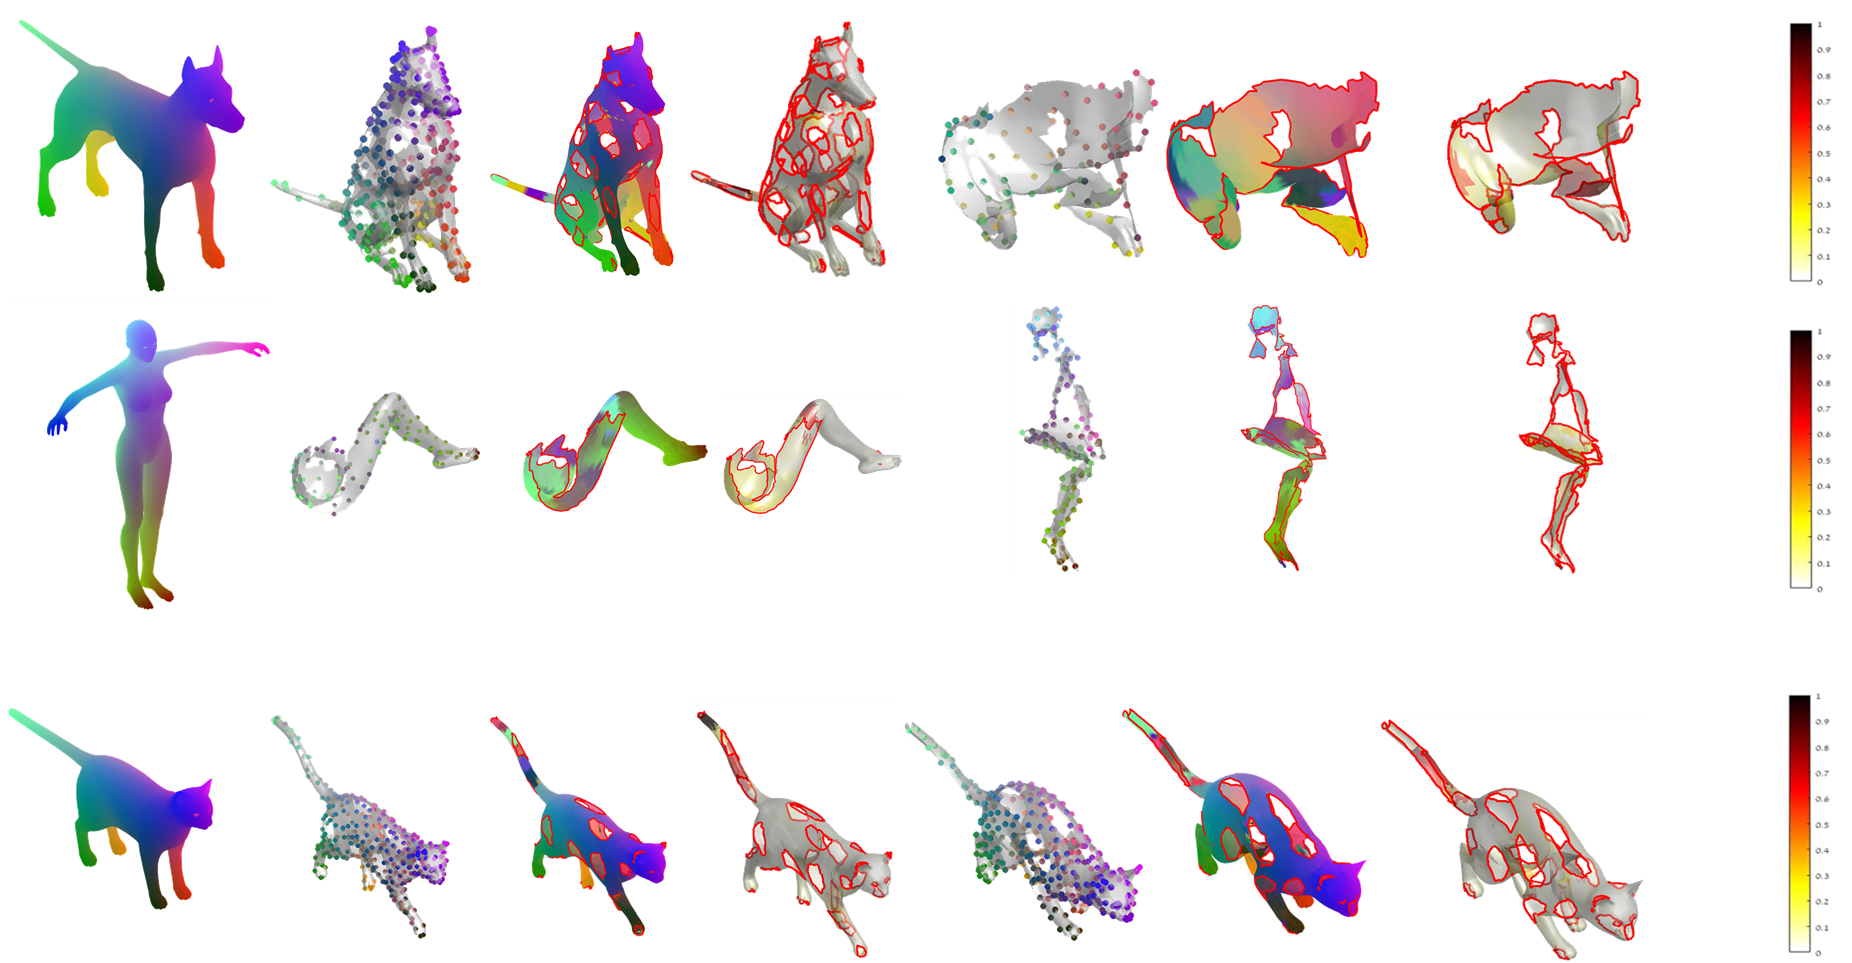
\includegraphics[width=1\textwidth]{figures/fail2.png}
	\caption{Some notable failure cases - most common is cat paw assignment - an extrinsic near symmetry gives rise to this phenomena. Closed fists on humanoids tends to cause a collapse of all fingers to a single finger. In the holes extreme partiality makes the geodesic distances break even over short distances.}
\end{figure*}
{\small
	\bibliographystyle{ieee}
	\bibliography{egbib}
}
\end{document}
